  \begin{tabular}{l l l l}
    \fbox{{\eq}-1}
    &
    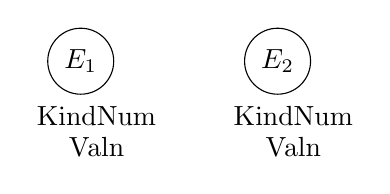
\begin{tikzpicture}[baseline]
      \node [draw,circle] (1) {$E_1$};
      \node [below of=1,yshift=2ex,xshift=2mm] (11) {\earsattr{Kind}{Num}};
      \node [below of=11,yshift=4ex] (12) {\earsattr{Val}{n}};
      \node [draw,circle,right of=1,xshift=1.5cm] (2) {$E_2$};
      \node [below of=2,yshift=2ex,xshift=2mm] (21) {\earsattr{Kind}{Num}};
      \node [below of=21,yshift=4ex] (22) {\earsattr{Val}{n}};
    \end{tikzpicture}
    &
    \coloneq
    &
    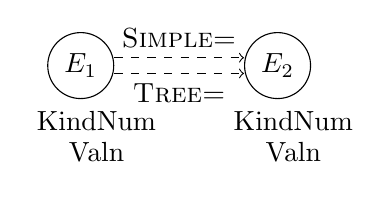
\begin{tikzpicture}[baseline]
      \node [draw,circle] (1) {$E_1$};
      \node [below of=1,yshift=2ex,xshift=2mm] (11) {\earsattr{Kind}{Num}};
      \node [below of=11,yshift=4ex] (12) {\earsattr{Val}{n}};
      \node [draw,circle,right of=1,xshift=1.5cm] (2) {$E_2$};
      \node [below of=2,yshift=2ex,xshift=2mm] (21) {\earsattr{Kind}{Num}};
      \node [below of=21,yshift=4ex] (22) {\earsattr{Val}{n}};

      \draw[->,dashed, transform canvas={yshift=1mm}] (1) -- node[above] {\textsc{Simple=}} (2);
      \draw[->,dashed, transform canvas={yshift=-1mm}] (1) -- node[below] {\textsc{Tree=}} (2);
    \end{tikzpicture}
  \end{tabular}

  \hdash

  \begin{tabular}{l l l l}
    \fbox{{\eq}-2}
    &
    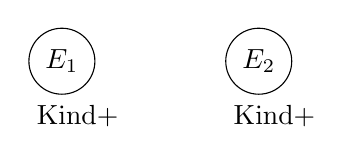
\begin{tikzpicture}[baseline]
      \node [draw,circle] (1) {$E_1$};
      \node [below of=1,yshift=2ex,xshift=2mm] (11) {\earsattr{Kind}{+}};
      \node [draw,circle,right of=1,xshift=1.5cm] (2) {$E_2$};
      \node [below of=2,yshift=2ex,xshift=2mm] (21) {\earsattr{Kind}{+}};
    \end{tikzpicture}
    &
    \coloneq
    &
    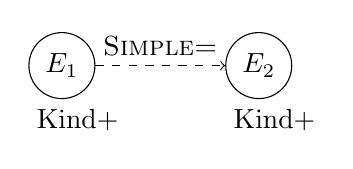
\begin{tikzpicture}[baseline]
      \node [draw,circle] (1) {$E_1$};
      \node [below of=1,yshift=2ex,xshift=2mm] (11) {\earsattr{Kind}{+}};
      \node [draw,circle,right of=1,xshift=1.5cm] (2) {$E_2$};
      \node [below of=2,yshift=2ex,xshift=2mm] (21) {\earsattr{Kind}{+}};

      \draw[->,dashed] (1) -- node[above] {\textsc{Simple=}} (2);
    \end{tikzpicture}
  \end{tabular}

\hdash

  \begin{tabular}{l l l l}
    \fbox{{\eq}-3}
    &
    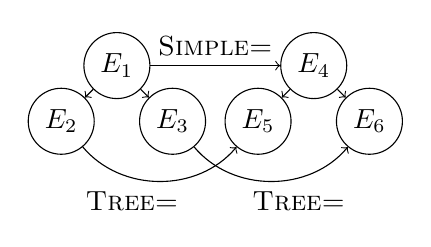
\begin{tikzpicture}[baseline]
      \node [draw,circle] (1) {$E_1$};
      \node [draw,circle,below left of=1] (2) {$E_2$};
      \node [draw,circle,below right of=1] (3) {$E_3$};
      \node [draw,circle,right of=1,xshift=1.5cm] (4) {$E_4$};
      \node [draw,circle,below left of=4] (5) {$E_5$};
      \node [draw,circle,below right of=4] (6) {$E_6$};

      \draw[->] (1) -- node[above] {\textsc{Simple=}} (4);
      \draw[->] (1) -- (2);
      \draw[->] (1) -- (3);
      \draw[->] (2) edge[bend right=50] node[below,xshift=-1em] {\textsc{Tree=}} (5);
      \draw[->] (3) edge[bend right=50] node[below,xshift=1em] {\textsc{Tree=}} (6);
      \draw[->] (4) -- (5);
      \draw[->] (4) -- (6);
    \end{tikzpicture}
    &
    \coloneq
    &
    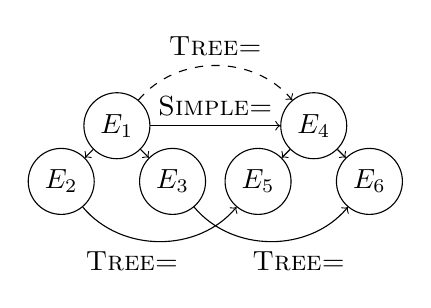
\begin{tikzpicture}[baseline]
      \node [draw,circle] (1) {$E_1$};
      \node [draw,circle,below left of=1] (2) {$E_2$};
      \node [draw,circle,below right of=1] (3) {$E_3$};
      \node [draw,circle,right of=1,xshift=1.5cm] (4) {$E_4$};
      \node [draw,circle,below left of=4] (5) {$E_5$};
      \node [draw,circle,below right of=4] (6) {$E_6$};

      \draw[->] (1) -- node[above] {\textsc{Simple=}} (4);
      \draw[->] (1) -- (2);
      \draw[->] (1) -- (3);
      \draw[->] (2) edge[bend right=50] node[below,xshift=-1em] {\textsc{Tree=}} (5);
      \draw[->] (3) edge[bend right=50] node[below,xshift=1em] {\textsc{Tree=}} (6);
      \draw[->] (4) -- (5);
      \draw[->] (4) -- (6);
      \draw[->,dashed] (1) edge[bend left=50] node[above] {\textsc{Tree=}} (4);
    \end{tikzpicture}
  \end{tabular}
